Let 
\begin{align}
 \vec{A}=c\myvec{\cos B\\\sin B},\vec{B}=\myvec{0\\0},\vec{C}=\myvec{a\\0}   
 \end{align}

\begin{align}
\because \angle C = 30^{\degree},
\end{align}
By law of sines
\begin{align}
\frac{\sin A}{a} &=\frac{\sin B}{b}=\frac{\sin C}{c}
\\
\implies c &=\frac{7{\sin 30^{\degree}}}{\sin 105^{\degree}}
\\
c &=3.62
\end{align}
and 
\begin{align}
 \vec{A} &=c\myvec{\cos B\\\sin B}
 \\
  &=\myvec{2.55\\2.55}
 \end{align}
Thus, the vertices of given $\triangle ABC$ are
\begin{align}
\vec{A}=\myvec{2.55\\2.55},\vec{B}=\myvec{0\\0},\vec{C} =\myvec{7\\0}
\end{align}
and  $\triangle ABC$ is plotted in Fig.  \ref{constr/5/fig:triangle ABC}.
%
\begin{figure}[!ht]
\centering
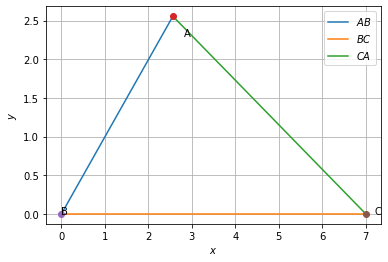
\includegraphics[width=\columnwidth]{solutions/triangle/5/Assignment1 (1)/figure.png}
\caption{$\triangle ABC$}
 \label{constr/5/fig:triangle ABC}
\end{figure}    
